% !TEX root = ../PhD Thesis.tex
\chapter{CompBio app server}
\label{chap:app-server}

Since I started building psichomics, I wanted to make it accessible as an online web app, allowing users to have the latest version at their fingerprints, without having to worry about installing and updating R, Bioconductor, psichomics and all their dependencies.
%It can take an hour to install psichomics from scratch and the command line may scare the end-users for whom psichomics was created. 
Following the first release of psichomics in Bioconductor 5 years ago, that vision finally came true.

One of our lab's ambitious goals is to develop interactive visual tools to explore biological data. These tools need to be intuitive enough to be used by everyone, no matter their computational background. To turn that into reality, I set up the CompBio app server, a Linux virtual machine that hosts multiple Shiny apps, including psichomics and cTRAP, as well as dashboards from my lab colleagues. The app server is publicly accessible at \url{https://compbio.imm.medicina.ulisboa.pt}.

% TODO: link to GitHub repo
% TODO: write specs of the app server?

CompBio is built using Docker Compose, a program that manages multiple Docker containers simultaneously, and is composed by the following intercommunicating services (\fullref{fig:architecture}):

\begin{figure}[!h]
  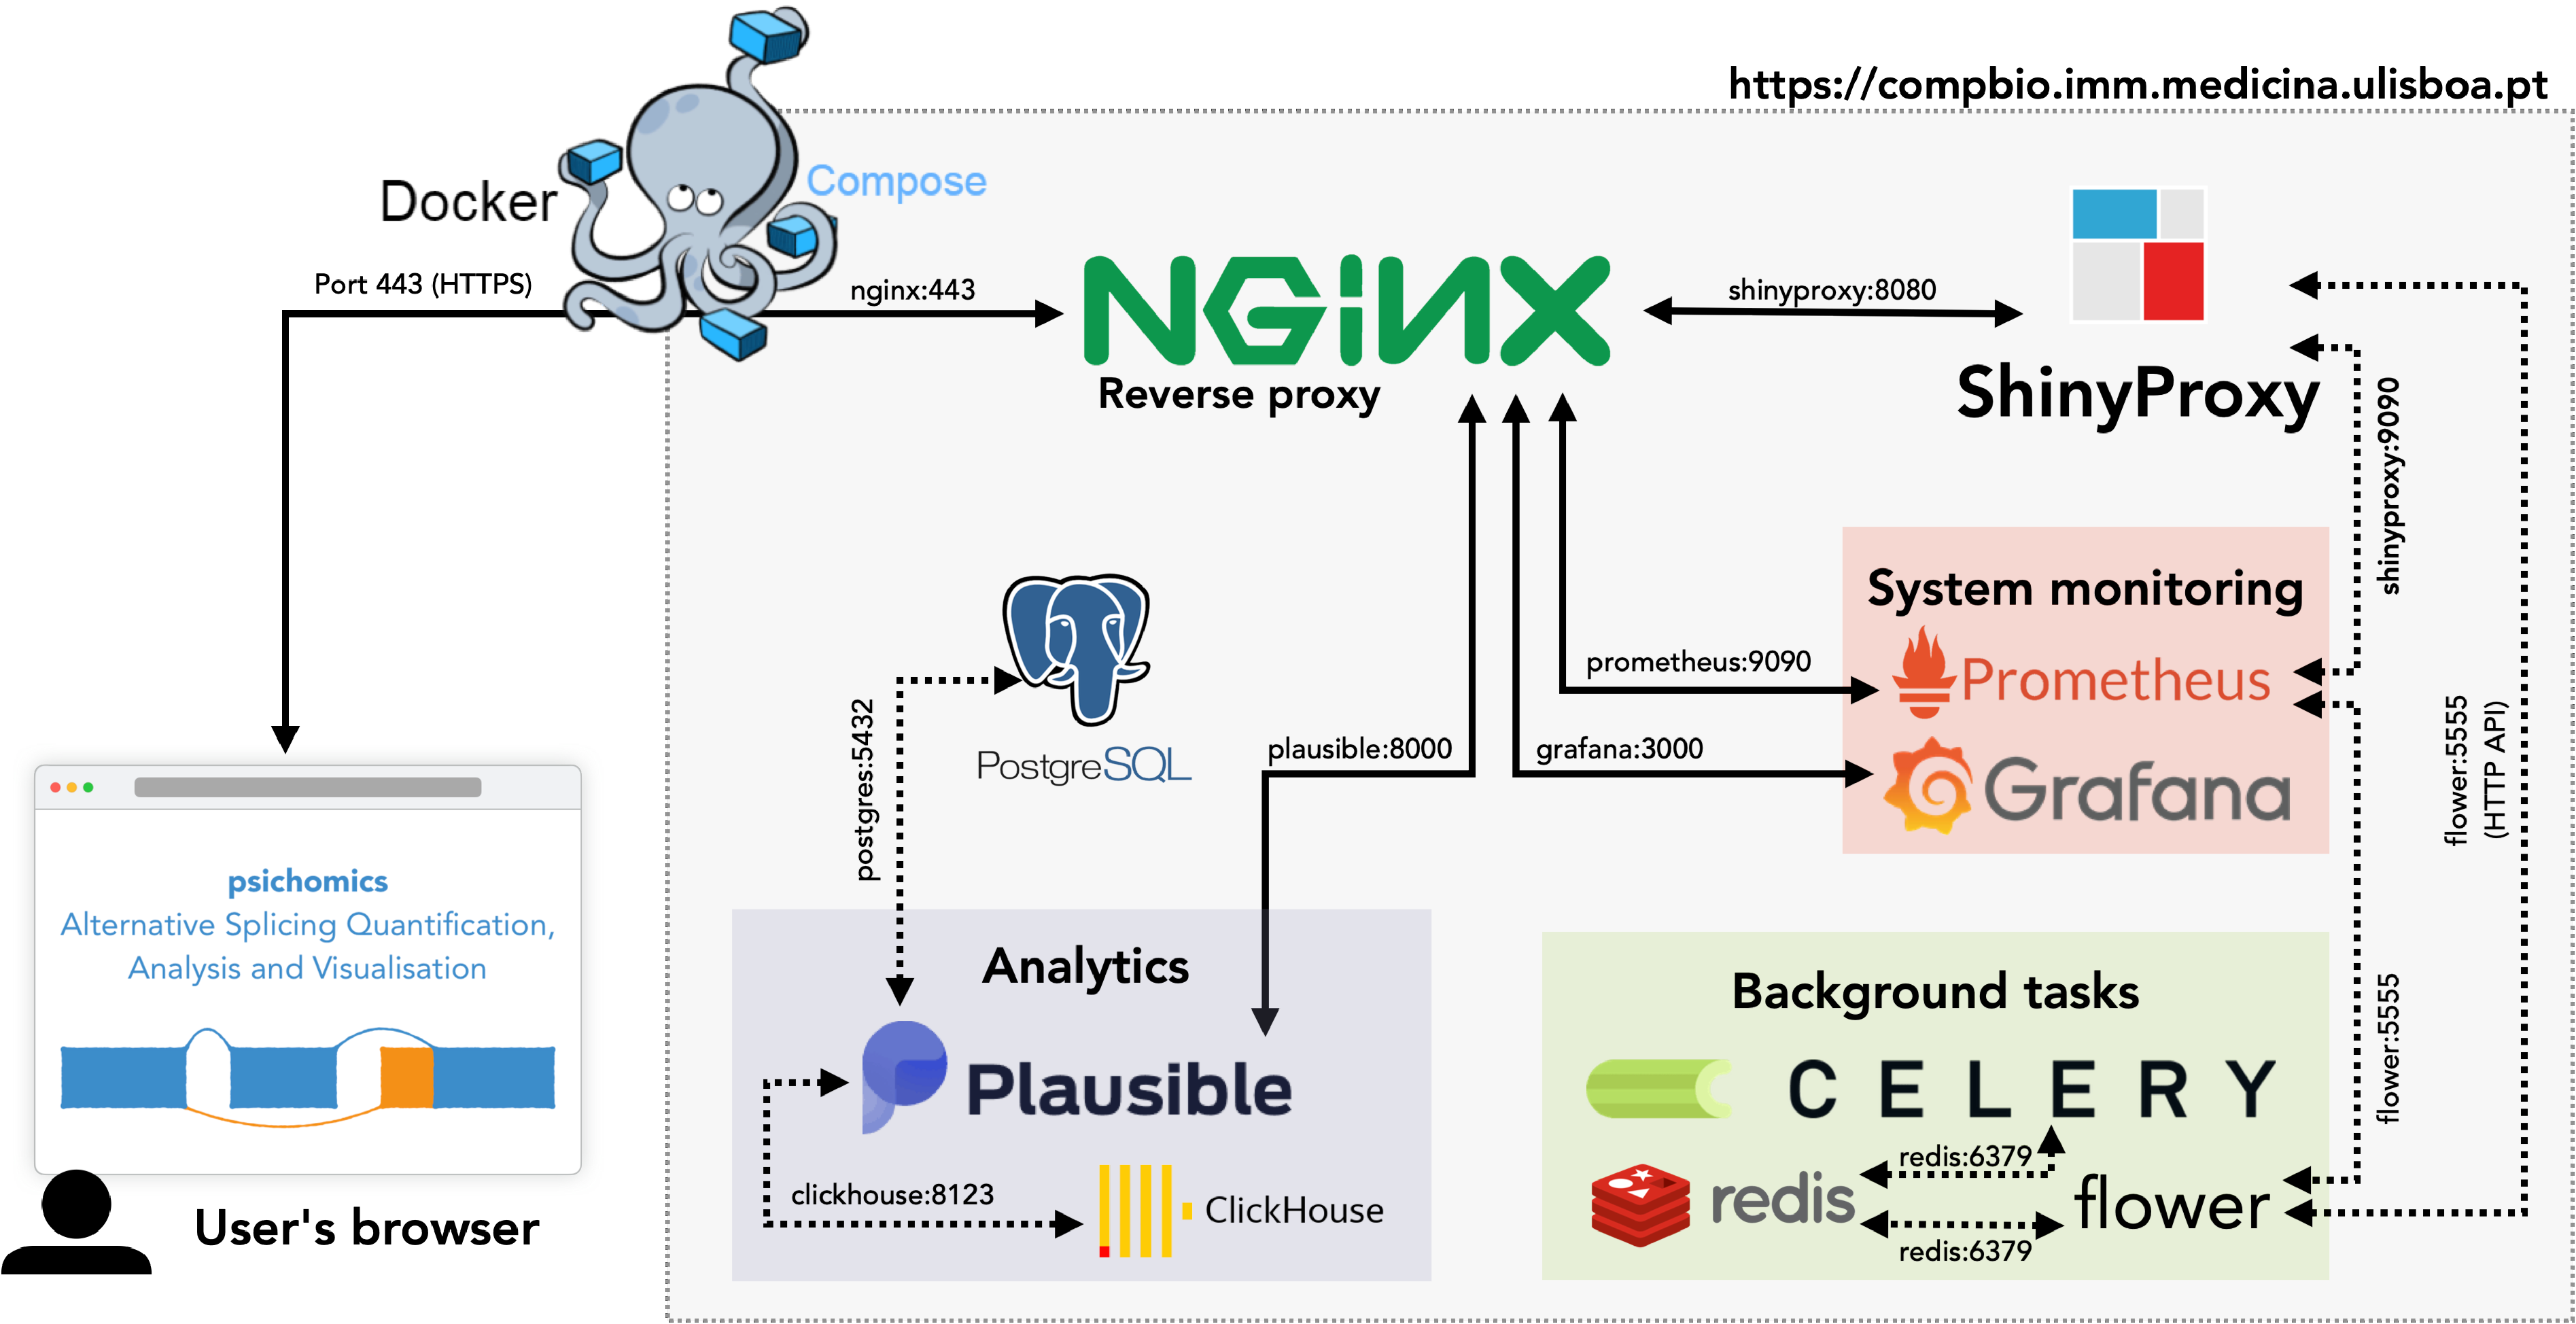
\includegraphics[width=1\textwidth]{images/app-server/architecture}
  \centering
  \caption[App server architecture]{\textbf{App server architecture is based on Docker Compose.} All services are provided via Docker images and communicate with each other via a Docker-created network using the name of the service and a specific port (e.g. Nginx communicates with ShinyProxy via \texttt{shinyproxy:8080}). The groups  (analytics, system monitoring and background tasks) are strictly conceptual.}
  \label{fig:architecture}
\end{figure}

\begin{itemize}
	\item \textbf{ShinyProxy} to serve web apps in R/Shiny and Python.
	\item \textbf{Nginx} as a reverse proxy, serves as an intermediary between the user requests and the server. Nginx is responsible to return what is shown to the user, to ensure HTTPS traffic is encrypted via SSL certificates, serve publicly available files and show a custom error page if ShinyProxy is not responding (e.g. temporarily down or overloaded).
	\item \textbf{Celery}, \textbf{Redis} and \textbf{Flower} to run background tasks.\footnote{More information in \fullref{sec:ctrap-web}}
	\item \textbf{Plausible}, \textbf{PostgreSQL} and \textbf{ClickHouse} for website analytics (i.e. track visitor metrics).
	\item \textbf{Prometheus} and \textbf{Grafana} to register and monitor server resources.
	\item \textbf{RStudio Web} to run R sessions and test features (not used in production).
\end{itemize}


\section{Docker Compose}

In Docker Compose, applications are run isolated from others in their own Docker containers, allowing to easily update or replace them without affecting other system components. All services spawned in Docker Compose are Docker images: either pre-created (e.g. official Docker images from Docker Hub) or created when starting all services based on a Dockerfile. CompBio can run in any Linux\footnote{Some services may require a different configuration to run in other operative systems.} machine with only Docker and Docker Compose installed, thus making the setup easily portable across different computers and requiring minimal user intervention.

A single file (\texttt{docker-compose.yml}) can be used to configure the applications.  The configuration of each service depends on the specific application and can be found either in \texttt{docker-compose.yml} or in the local directory. For organisation purposes, the local directory was organised by folders named after each service, where each folder stores files (e.g. Dockerfile, configuration and data) associated with the respective application (\fullref{fig:file-structure}).

\begin{figure}[!h]
  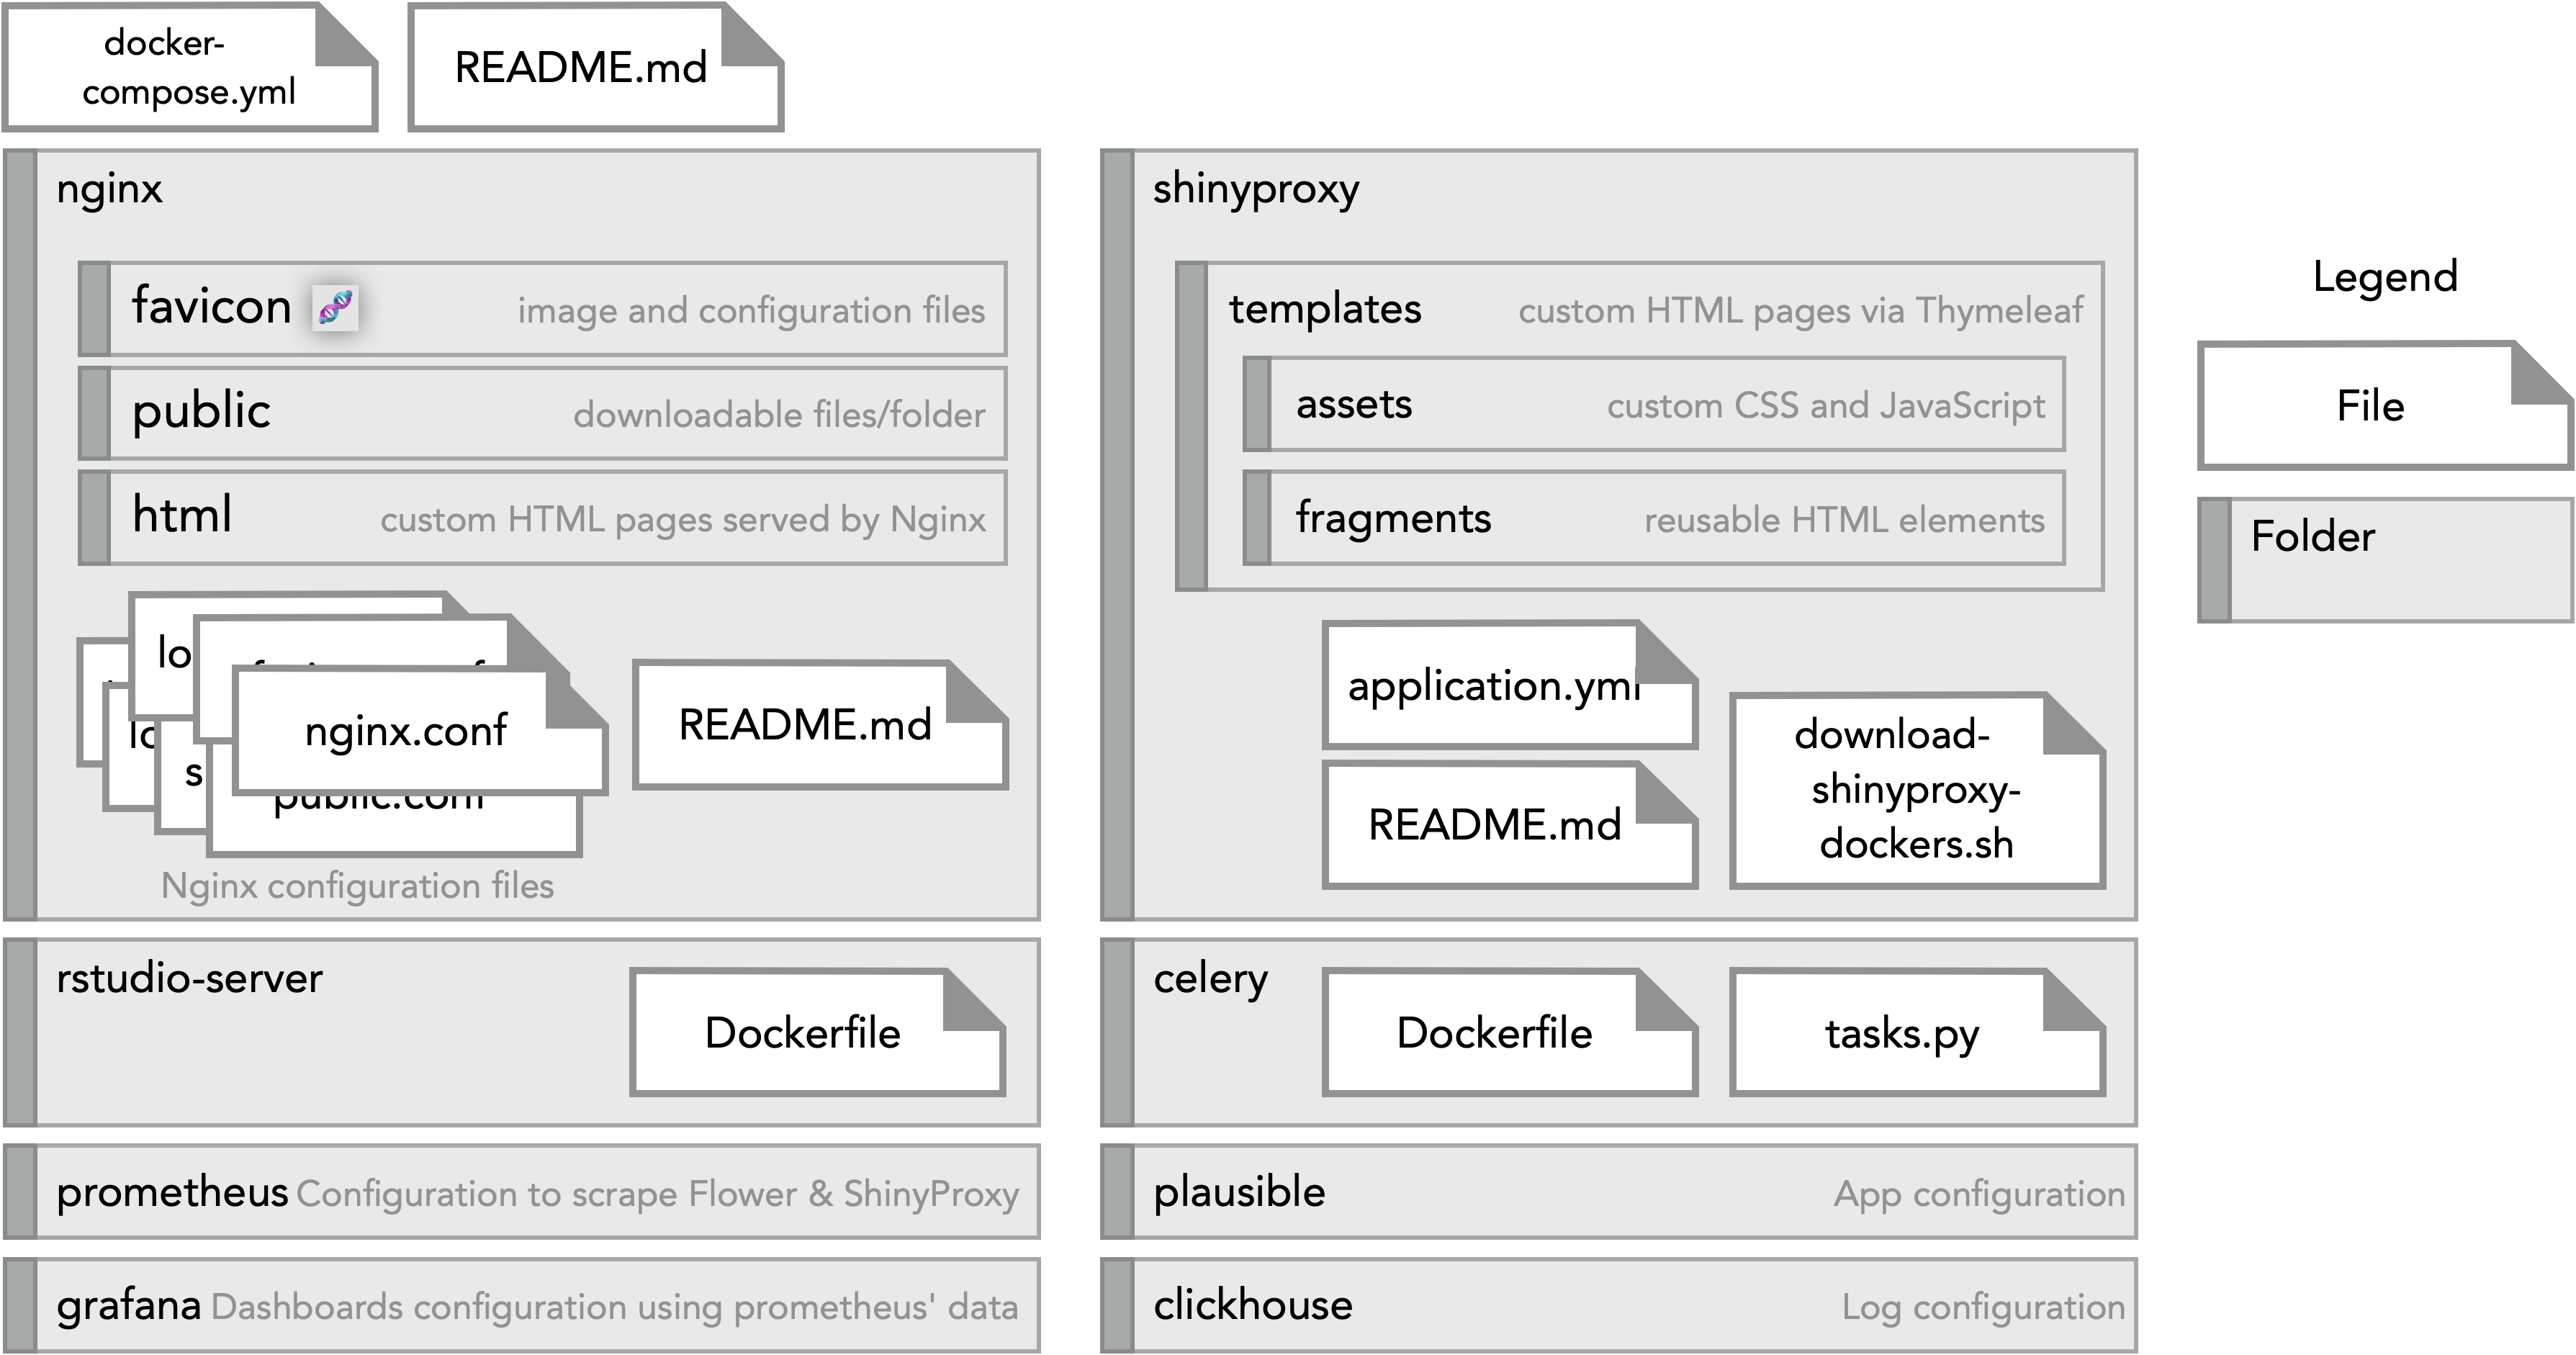
\includegraphics[width=1\textwidth]{images/app-server/file-structure}
  \centering
  \caption[App server's file structure]{\textbf{App server's file structure.} Visual representation of the file/directory structure of the CompBio app server. Each folder contains files associated with a specific service. Folders \texttt{rstudio-server} and \texttt{celery} contain Dockerfiles for building Docker images of the respective services.}
  \label{fig:file-structure}
\end{figure}

Data from containers are preserved in volumes to avoid data loss when restarting services. Docker volumes are mounted when starting the \texttt{docker-compose.yml} project. Although Docker containers destroy all data within, specific directories are mounted in Docker volumes to be stored in the long-term (such as databases).

A single command is enough to build Docker images from available Dockerfiles, download Docker images from Docker Hub and start up every service in detached mode: \texttt{docker-compose up -d --build}.

Multiple \texttt{docker-compose} commands allow to manage the services. For instance, it is possible to restart single services (without affecting other programs), specially useful when altering the configuration of a service. However, changes to \texttt{docker-compose.yml} are only applied after restarting all services by shutting down all services with \texttt{docker-compose down}.

\section{ShinyProxy}

ShinyProxy is an open-source program that deploys R/Shiny and Python apps via Docker. When a user starts an app, ShinyProxy creates a new Docker container exclusively for that user. The containers are automatically terminated 30 minutes (by default) after the last user interaction.

Adding new apps to the system is as simple as pulling the Docker image of the app in the server and adding them to the ShinyProxy configuration file.

\subsection{Features}

ShinyProxy offers multiple built-in features, including:

\begin{itemize}
	\item \textbf{Usage statistics:} many ShinyProxy metrics (including app usage time, app failures and user numbers) are collected with Prometheus and visualised using Grafana.
    \item \textbf{App recovery:} when restarting ShinyProxy, ShinyProxy-initiated Docker containers continue running in the background and are attached once ShinyProxy finishes loading, minimising issues related with server maintenance. The apps will be unavailable while ShinyProxy is not running. For more information, please read \url{https://shinyproxy.io/documentation/app-recovery}.
    \item \textbf{User authentication:} authentication with multiple methods, including social login via GitHub, LinkedIn, Google, etc. However, user authentication requires all visitors to login before continuing. As we prefer users to be able to anonymously access our apps, this feature is currently disabled.
    \item \textbf{User sessions:} user data can be stored in user-specific folders. As the sessions are only accessible when the Docker container is already attached to the volumes, this allows for complete isolation from other user folders. However, this feature works best with user authentication enabled (otherwise, random identifiers are used for each visitor and requires custom logic to load data between computers).
	\item \textbf{Multiple app instances:} users can open and manage multiple app instances simultaneously (not currently enabled in the app server); more information at \url{https://shinyproxy.io/documentation/ui/#using-multiple-instances-of-an-app}.
\end{itemize}

\subsection{Progress bar when opening apps}

When ShinyProxy is loading an app, a spinning wheel is shown as a loading indicator. This may work fine for apps that take 5 seconds to load, but anything longer may give the impression that there is something wrong with loading the webpage. To avoid that feeling, I added a progress bar that fills up with time to replace the spinning wheel.

However, if the progress bar fills up too fast, it will not have the desired effect. By default, the progress bar takes 5 seconds to fill (as most apps take that much time to launch in ShinyProxy), but the time is customisable for specific apps. For instance, psichomics usually takes 20 seconds to start, whereas cTRAP takes 15 seconds. When the app is ready, the progress bar fades into the app, no matter the progress shown.

To create this progress bar, \verb|shinyproxy/templates/app.html| was edited to remove the spinning wheel and to include an empty progress bar. The progress bar's width is changed from 0\% to 100\% a millisecond afterwards. To make this transition smooth (instead of filling the bar directly), the progress bar is given two classes for each app: classes \verb|progress-bar| and a custom \verb|progress-{appID}|, where \verb|appID| is a specific app identifier. The CSS file (\verb|shinyproxy/templates/assets/shinyproxy.css|) has a rule for class \verb|progress-bar| to perform a 5-second ease in-and-out animation when changing the width of the progress bar. This rule can be superseded by a custom \verb|progress-{appID}| with a different time interval of choice. In the case of psichomics, the CSS file includes a custom rule for its progress bar's 20-second transition: \verb|.progress-bar { transition: width 20s ease-in-out; }|.

\section{Nginx}

Nginx is a reverse proxy, i.e. an intermediary that decides what is shown to the user depending on the URL visited.

% akin to those switchboard operators seen in the old movies

Nginx is also used for ensuring encrypted HTTPS traffic via SSL certificates.

A public folder is available via Nginx.

In case ShinyProxy is down, Nginx will serve a custom error page stating that the server is down probably because of ShinyProxy. This is informative enough to end-users that know they should wait to refresh the page in a moment and also to admins that will understand that ShinyProxy is temporarily down (this can happen because of multiple reasons, such as a restart of the service or overloading).

\section{Plausible}

Plausible is an open-source, privacy-focused web analytics tool that collects traffic metrics for multiple websites and provides them via an interactive dashboard. CompBio runs the self-hosted version of Plausible. All of Plausible metrics (e.g., visitor numbers, total page views and session duration) are anonymously aggregated without cookies, thus avoiding individual tracing.

% plausible vs google analytics
The best thing about using the self-hosted version of Plausible is that the data tracked of the users is minimal, is harder to individually trace (thus protecting user privacy) and complies with privacy laws (GDPR, CCPA and PECR) because no personal data is collected. This is in stark contrast with Google Analytics.

\section{Server Maintenance}

% TODO: Improve server security: see ShinyProxy security best practices
% TODO: Run Docker images as rootless
% TODO: Change service passwords

CompBio is a web server that hosts Shiny applications and is publicly accessible by everyone online. This makes our server a target for potential security attacks. In order to mitigate such vulnerabilities, it is crucial to update user-facing programs (Docker, Docker Compose, Nginx and ShinyProxy), while components that are not directly available to end-users should be updated when possible. As updates may contain breaking changes that hamper website functionality, it is recommended to read change logs related to new software versions to pinpoint potential issues before updating.

% https://www.sciencedirect.com/science/article/pii/S2352484721007289#b71
% https://doi.org/10.1145/3038923
% https://www.tandfonline.com/doi/full/10.1080/19393555.2020.1853855?casa_token=EpT3lJflBXAAAAAA%3AaS5ePDNIcAPfL6MsMoKrI0s4sDtjyGNvGICZiz2Ywvnf7E2vtokORb073GUi9eilZiUCFOAqhIY

Updates to Docker and Docker Compose need to be performed by an administrator using Linux's \texttt{apt-get} command. Docker images of the server (including Nginx and ShinyProxy), on the other hand, require a user in the \texttt{docker} group to pull the latest Docker images from Docker Hub and edit the versions of the Docker images used in \texttt{docker-compose.yml} accordingly. Afterwards, the app server services are restarted with \texttt{docker-compose down \&\& docker-compose up -d --build}. Another advantage of using Docker Compose is that if something goes wrong with the updated Docker images, we simply need to edit \texttt{docker-compose.yml}, indicate a previous version of the software to run and restart the services.

% root + Docker